\graphicspath{{./figures/}}
\title{}
\date{}
\begin{document}
\begin{frame}
    \titlepage
\end{frame}

\begin{frame}{last time}
    \begin{itemize}
    \item coverage-guided fuzzing
        \begin{itemize}
        \item random tests based on set of base tests
        \item new path taken: add test to set of base tests
        \end{itemize}
    \item complete (finds any problem) v sound (problems found really problems)
    \item static analysis
        \begin{itemize}
        \item \textit{abstract interpretation}: summary values e.g. allocated/freed
        \item approximations to avoid analyzing complex if statements, etc.
        \end{itemize}
    \end{itemize}
\end{frame}

\subsection{example: model for use-after-free, with loop}
    % FIXME: hilite: repeated states allow compression
\usetikzlibrary{arrows.meta}
\begin{frame}[fragile,label=useAfterFree3]{checking use-after-free (3)}
    \lstset{
        language=C,style=script,
        moredelim={**[is][\btHL<2>]{~2~}{~end~}},
    }
\begin{tikzpicture}
\node[anchor=north east] at (-.2, 0) {
\begin{lstlisting}
void someFunction() {
    int *quux = malloc(sizeof(int));
    ...
    // A
    do {
        // B
        ...
        if (anotherFunction()) {
            free(quux);
            // C
        }
        ...
        // D
    } while (complexFunction());
    ...
    // E
    *quux++;
    ...
}
\end{lstlisting}
};
    \tikzset{flow/.style={draw,thick,font=\fontsize{9}{10}\selectfont,anchor=north west},
    flowLine/.style={thick,-Latex},
    flowLineB/.style={very thick,dotted,-Latex},
    }
    \begin{scope}[y=0.8cm]
        \begin{visibleenv}<1->
        \node[flow] (A) at (0, 0) { A: \textit{allocated} };
        \node[flow,alt=<3>{red}{},alt=<1-2>{dashed}] (B) at (1, -1) { B (from \textit{allocated}): \textit{allocated} };
        \draw[flowLine] ([xshift=.5cm]A.south west) |- ([yshift=.1cm]B.west);
        \end{visibleenv}
        \begin{visibleenv}<2->
        \node[flow] (C1) at (1, -2) { C (from \textit{allocated}): quux: \textit{freed} };
            \node[flow,alt=<1-4>{dashed}{}] (D1) at (1, -3) { D (from \textit{freed}): \textit{freed} };
        \node[flow] (E1) at (2, -4) { E (from \textit{freed}): USE-AFTER-FREE };
        \draw[flowLine] ([yshift=-.1cm]B.west) -- ++(-.2cm, 0cm) |- ([yshift=.1cm]C1.west);
        \draw[flowLine] ([yshift=-.1cm]C1.west) -- ++(-.2cm, 0cm) |- ([yshift=.1cm]D1.west);
        \draw[flowLine] ([yshift=-.1cm]D1.west) -- ++(-.2cm, 0cm) |- ([yshift=.1cm]E1.west);
        \end{visibleenv}
        \begin{visibleenv}<3->
        \node[flow,alt=<3>{dashed}{}] (D2) at (1, -5) { D (from \textit{allocated}): \textit{allocated} };
        \draw[flowLine,alt=<3>{red}{}] ([yshift=-.1cm]B.west) -- ++(-.3cm, 0cm) |- ([yshift=.1cm]D2.west);
        \node[flow] (E2) at (2, -6) { E (from \textit{allocated}): ok };
        \draw[flowLine,alt=<3>{red}{}] ([yshift=-.1cm]D2.west) -- ++(-.2cm, 0cm) |- ([yshift=.1cm]E2.west);
        \end{visibleenv} 
        \begin{visibleenv}<4->
        \draw[flowLineB,alt=<4>{red}{}] ([yshift=-.1cm]D2.east) -- ++(2.5cm, 0cm) |- ([yshift=.1cm]B.east);
        \end{visibleenv} 
        \begin{visibleenv}<5->
            \node[flow,alt=<5>{dashed}{}] (B2) at (1, -7) { B (from \textit{freed}): \textit{freed} };
            \draw[flowLine,alt=<5>{red}{}] ([yshift=-.1cm]D1.west) -- ++(-.8cm, 0cm) |- ([yshift=.1cm]B2.west);
            \node[flow] (C2) at (1, -8) { C (from \textit{freed}): DOUBLE-FREE };
            \draw[flowLine] ([yshift=-.1cm]B2.west) -- ++(-.8cm, 0cm) |- ([yshift=.1cm]C2.west);
        \end{visibleenv} 
        \begin{visibleenv}<6->
            \draw[flowLineB,alt=<6>{red}{}] ([yshift=-.1cm]B2.east) -- ++(3cm, 0cm) |- ([yshift=.2cm]D1.east);
        \end{visibleenv}
    \end{scope}
\end{tikzpicture}
\end{frame}

\begin{frame}{result from clang's scan-build}
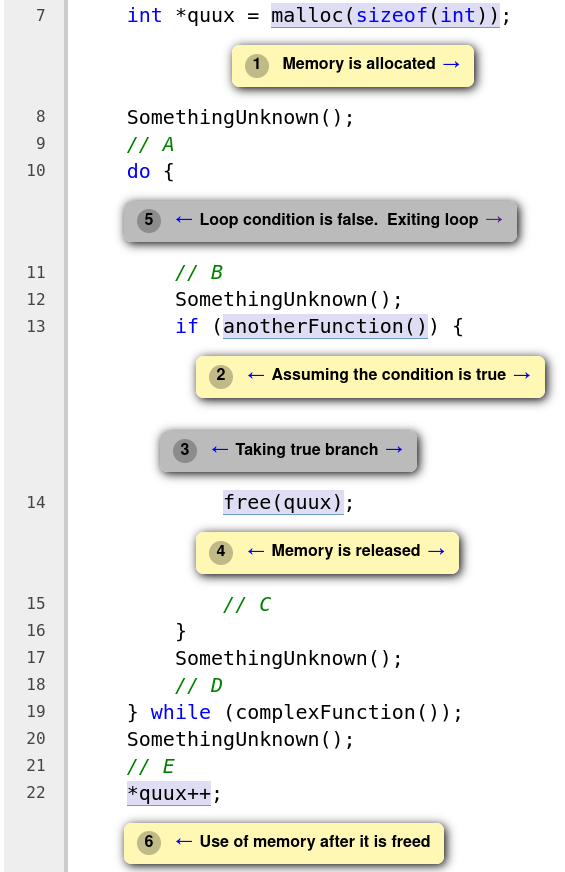
\includegraphics[height=0.9\textheight]{../static/scan-build-uaf-example3a}
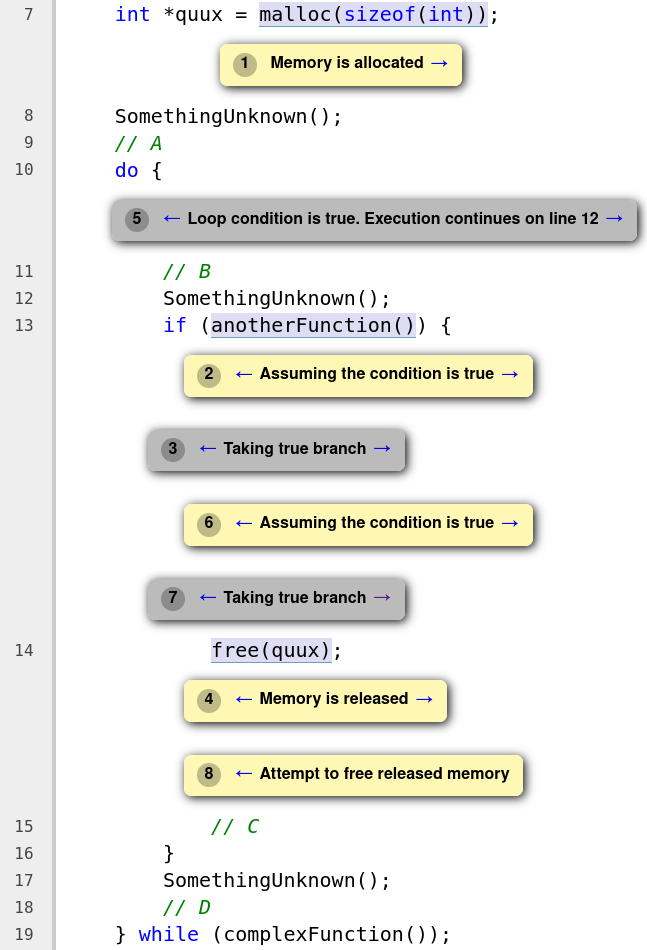
\includegraphics[height=0.9\textheight]{../static/scan-build-uaf-example3b}
\end{frame}


\subsection{example: model for array bounds}
\usetikzlibrary{arrows.meta}
\begin{frame}{checking for array bounds}
    \begin{itemize}
    \item can \textit{try} to apply same technique to array bounds
    \item but much more complicated/more likely to have false positives/negatives
    \vspace{.5cm}
    \item for each array or pointer track:  
        \begin{itemize}
        \item minimum number of elements before/after what it points to
        \end{itemize}
    \item for each integer track: 
        \begin{itemize}
        \item minimum bound
        \item maximum bound
        \end{itemize}
    \item similar analysis looking at paths?
    \end{itemize}
\end{frame}

\begin{frame}[fragile,label=bounds1]{checking array bounds (1)}
    \lstset{
        language=C,style=script,
        moredelim={**[is][\btHL<2>]{~2~}{~end~}},
    }
\begin{tikzpicture}
\node[anchor=north east] at (-.2, 0) {
\begin{lstlisting}
int array[100];
void someFunction(int foo) {
    // A
    if (foo > 100) {
        return;
    }
    // B
    array[foo] += 1;
}
\end{lstlisting}
};

    \tikzset{
        flow/.style={draw,thick,font=\fontsize{9}{10}\selectfont,anchor=north west},
        flowLine/.style={thick,-Latex},
    }
    \begin{scope}[y=1.2cm]
        \node[flow] (A) at (0, 0) { A: foo: $[-\inf, +\inf]$; array: indices [0, 99] };
        \node[flow] (B) at (0, -1) { B: foo: $[-\inf, +100]$; array: indices [0, 99] };
        \draw[flowLine] (A) -- (B);
    
    \begin{visibleenv}<2->
        \node[draw=red,very thick,fill=white,align=center] at (0, -4) {
            give warning about \texttt{foo == 100}? probably bug! \\
            give warning about \texttt{foo < 0}? maybe??
        };
    \end{visibleenv}
    \end{scope}
\end{tikzpicture}
\end{frame}

\begin{frame}[fragile,label=bounds2]{checking array bounds (2)}
    \lstset{
        language=C,style=script,
        moredelim={**[is][\btHL<2>]{~2~}{~end~}},
    }
\begin{tikzpicture}
\node[anchor=north east] at (-.2, 0) {
\begin{lstlisting}
int array[100];
void someFunction(int foo, bool bar) {
    int *p = array;
    // A
    p += 50;
    // B
    if (foo >= 50 || foo < 0) abort();
    // C
    if (bar) {
        foo = -foo;
    }
    // D
    p[foo] = 1;
}
\end{lstlisting}
};

    \tikzset{flow/.style={draw,thick,font=\fontsize{9}{10}\selectfont,anchor=north west},
    flowLine/.style={thick,-Latex}}
    \begin{scope}[y=1.2cm]
        \node[flow] (A) at (0, 0) { A: p: indices [0, 99]; foo: $[-\inf, +\inf]$ };
        \node[flow] (B) at (0, -1) { B: p: indices [-50, 49]; foo: $[-\inf, +\inf]$ };
        \node[flow] (C) at (0, -2) { C: p: indices [-50, 49]; foo: [0, 50] };
        \node[flow] (D1) at (-4, -3) { D (bar true): p: indices: [-50, 49]; foo: [-50, 0] } ;
        \node[flow,alt=<2>{draw=red}] (D2) at (1, -4) { D (bar false): p: indices: [-50, 49]; foo: [0, 50] };
        \draw[flowLine] (A) -- (B);
        \draw[flowLine] (B) -- (C);
        \draw[flowLine] (C) -- (D1);
        \draw[flowLine] (C) -- (D2);
    
    \begin{visibleenv}<2->
        \node[draw=red,very thick,fill=white,align=center] at (0, -6) {
            warn about possible out-of-bounds? 
        };
    \end{visibleenv}
    \end{scope}
\end{tikzpicture}
\end{frame}


\subsection{analysis for common insecure patterns}
\begin{frame}{common bug patterns}
    \begin{itemize}
    \item effectively detecting things like ``arrays are in bounds'' \\
        or ``values aren't used after being freed'' \\
        is not very reliable for large programs
    \item (but analysis tools are getting better)
    \vspace{.5cm}
    \item but static analysis tools shine for \myemph{common bug patterns}
    \end{itemize}
\end{frame}

\begin{frame}[fragile,label=suspectPatterns]{patterns clang's analyzer knows}
\begin{lstlisting}[language=C,style=smaller]
struct foo *p = malloc(sizeof(struct foo*)); // meant struct foo?
long *p = malloc(16 * sizeof(int)); // meant sizeof(long)?
\end{lstlisting}
\hrule
\begin{lstlisting}[language=C,style=smaller]
strncat(foo, bar, sizeof(foo));
\end{lstlisting}
\hrule
\begin{lstlisting}[language=C,style=smaller]
int *global;
int *foo() {
    int x;
    int *p = &x;
    ...
    global = p; // putting pointer to stack in global
    return p;    // returning pointer to stack
}
\end{lstlisting}
\end{frame}

\begin{frame}[fragile,label=suspectPatterns]{more suspect patterns }
    \begin{itemize}
    \item SpotBugs: Java static analysis tool
    \end{itemize}
\begin{lstlisting}[language=Java,style=smaller]
// pattern: connecting to database with empty password:
connection = DriverManager.getConnection(
    "jdbc:hsqldb:hsql://db.example.com/xdb" /* database ID */, 
    "sa" /* username */, "" /* password */);

// pattern: Sql.hasResult()'s second argument isn't a constant
Sql.hasResult(c, "SELECT 1 FROM myTable WHERE code='"+code+"'");

// pattern: new FileReader's argument comes from request
HttpRequest request = ...;
String path = request.getParameter("path");
BufferedReader r = new BufferedReader(
    new FileReader("data/" + path));
\end{lstlisting}
\end{frame}


\begin{frame}{preview: information flow}
    \begin{itemize}
    \item really common pattern we want to find: \\
        data from somewhere gets to dangerous place
        \begin{itemize}
        \item pointer to stack escapes function
        \item input makes it to SQL query, file name
        \end{itemize}
    \item we'll talk about it specially next
    \end{itemize}
\end{frame}

\subsection{summary / actual tools}
\begin{frame}[fragile,label=practic]{static analysis practicality}
    \begin{itemize}
    \item good at finding some kinds of bugs
        \begin{itemize}
        \item array out-of-bounds probably not one --- complicated tracking needed
        \end{itemize}
    \item excellent for ``bug patterns'' like:
\begin{lstlisting}
struct Foo* foo;
...
foo = malloc(sizeof(struct Bar));
\end{lstlisting}
    \item false positive rates are often 20+\% or more
    \item some tools assume lots of annotations
    \item not limited to C-like languages
    \end{itemize}
\end{frame}

\begin{frame}{static analysis tools}
    \begin{itemize}
    \item Coverity, Fortify --- commerical static analysis tools
    \item Splint --- unmaintained?
        \begin{itemize}
            \item written by David Evans and his research group in the late 90s/early 00s
        \end{itemize}
    \item FindBugs (Java)
    \item clang-analyzer --- part of Clang compiler
    \item Microsoft's Static Driver Verifier  --- required for Windows drivers:
        \begin{itemize}
            \item mostly checks correct usage of Windows APIs
        \end{itemize}
    \end{itemize}
\end{frame}



\section{information flow}
\begin{frame}{information flow}
    \begin{itemize}
    \item so far: static analysis concerned with control flow
    \item often, we're really worried about how \textit{data} moves
    \vspace{.5cm}
    \item many applications:
        \begin{itemize}
        \item does an array index depend on user input?
        \item does an SQL query depend on user input?
        \item does data sent over network depend on phone number?
        \end{itemize}
    \item \ldots
    \vspace{.5cm}
    \item can do this \textit{statically} (potential dependencies) \\
         or \textit{dynamically} (actual dependencies as program runs)
    \end{itemize}
\end{frame}


\subsection{data flow graph}
\begin{frame}[fragile,label=infoFlowExample1a]{information flow graph (1a)}
\begin{lstlisting}[language=Python,style=smaller]
def f(a, b, c):
    desc = 'a={},b={}'.format(a, b)
    if b > 10:
        y = a
    else:
        y = c
    w = y + a
    pair = (w, c)
    desc = desc + \
         ',pair={}'.format(pair)
    print(desc)
    return y
\end{lstlisting}
\begin{tikzpicture}[overlay,remember picture]
\node[anchor=north east] at ([xshift=-.25cm,yshift=-1cm]current page.north east) {
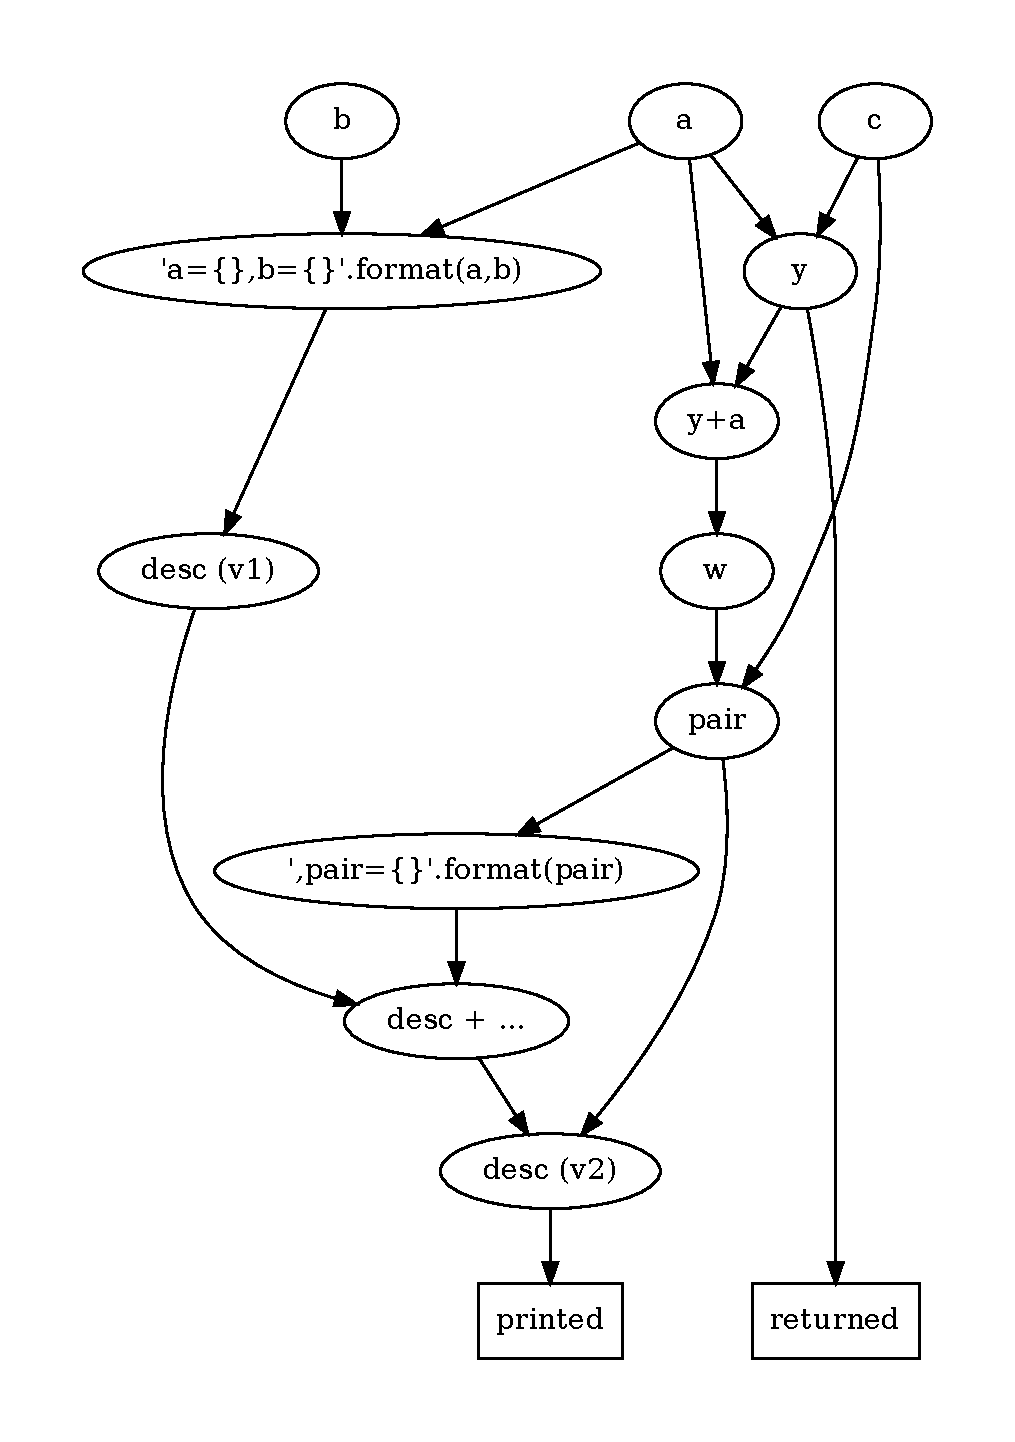
\includegraphics[width=0.4\textwidth]{../taint/info-flow-graph1}
};
\end{tikzpicture}
\end{frame}

\begin{frame}[fragile,label=infoFlowExample1b]{information flow graph (1b)}
\begin{itemize}
\item<2-> ex: does returned value depend on a, b, c?
\item<2-> ex: does value of pair depend on a, b, c?
\item<2-> ex: does printed value depend on a, b, c?
\end{itemize}
\begin{tikzpicture}[overlay,remember picture]
\node[anchor=north east] at ([xshift=-.25cm,yshift=-1cm]current page.north east) {
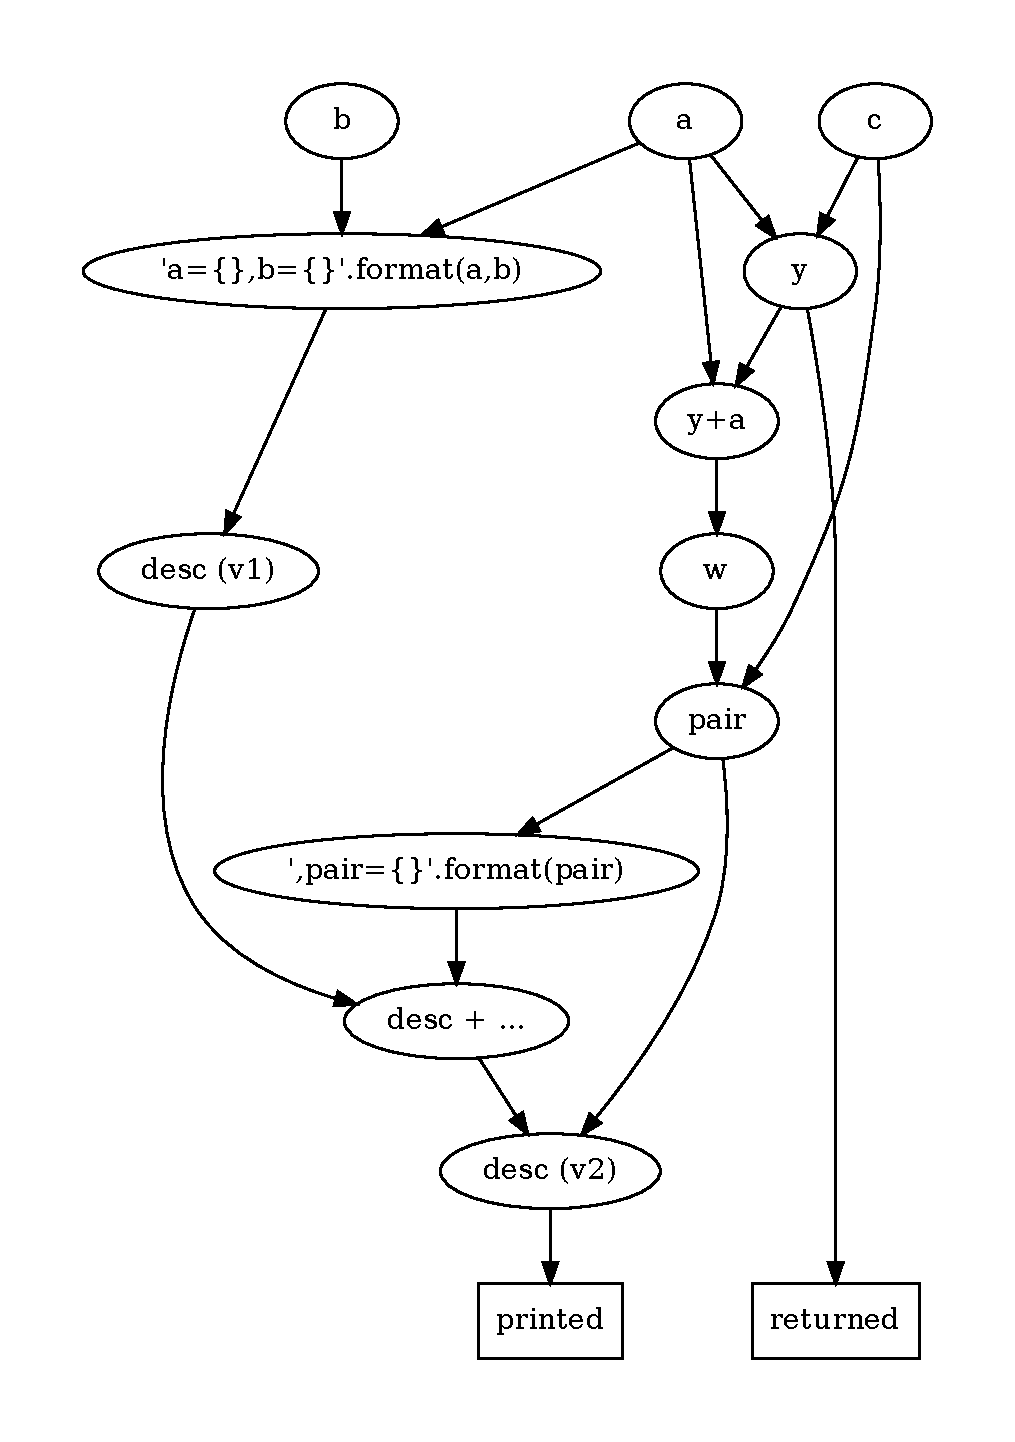
\includegraphics[width=0.4\textwidth]{../taint/info-flow-graph1}
};
\end{tikzpicture}
\end{frame}


\subsection{control flow versus information flow} 
\begin{frame}[fragile,label=infoFlowVControlFlow]{information flow and control flow}
\begin{lstlisting}[language=Python,style=smaller]
def f(a, b, c):
    if b > 10:
        y = a
    else:
        y = c
    return y
\end{lstlisting}
\begin{itemize}
\item Q: which is better \ldots
    \begin{itemize}
    \item if we're trying to see if user input makes it to SQL query?
    \item if we're trying to determine if private info goes out over network?
    \end{itemize}
\end{itemize}
\begin{tikzpicture}[overlay,remember picture]
\node[anchor=north east] (main) at ([xshift=-.25cm,yshift=-1cm]current page.north east) {
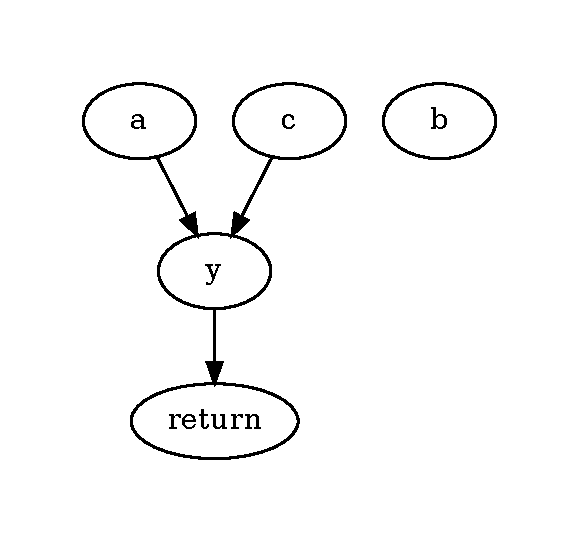
\includegraphics[width=0.3\textwidth]{../taint/info-flow-graph2}
};
\node[anchor=north east] (second) at (main.north west) {
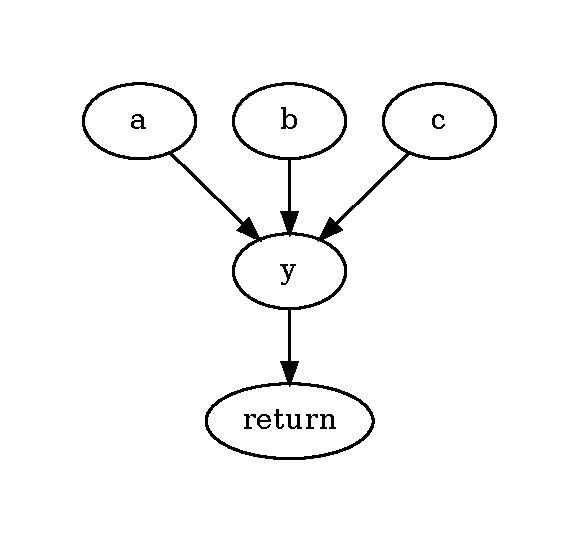
\includegraphics[width=0.3\textwidth]{../taint/info-flow-graph2b}
};
\end{tikzpicture}
\end{frame}


\subsection{sources and sinks}
\begin{frame}{sources and sinks}
    \begin{itemize}
    \item needed choose \textit{sources} (so far: function arguments) \\
          and \textit{sinks} (so far: print, return)
    \item choice depends on application
    \item SQL injection: 
        \begin{itemize}
        \item sources: input from network
        \item sinks: SQL query functions
        \end{itemize}
    \item private info leak:
        \begin{itemize}
        \item sources: private data: phone number, message history, email, \ldots
        \item sinks: network output
        \end{itemize}
    \end{itemize}
\end{frame}


\subsection{challenges for data flow}
\begin{frame}[fragile,label=dFlowChallenges1]{static info flow challenges (1)}
\begin{tikzpicture}
\node (left) {
\begin{lstlisting}[language=Python,style=smaller]
# Python example
def stash(a):
    global y
    y = a
x = [0,1,2,3]
stash(x)
x[2] = input()
print(y[2])
\end{lstlisting}
};
\node[anchor=north west] at ([xshift=3cm]left.north east) {
\begin{lstlisting}[language=C++,style=smaller]
// C example
int *y;
void stash(int *a) {
    y = a;
}
int main() {
    int x[3];
    stash(x);
    y[2] = GetInput();
    printf("%d\n",x[2]);
}
\end{lstlisting}
};
\end{tikzpicture}
\begin{itemize}
\item same points-to problem with static analysis
\item need to realize that x[2] and y[2] are the same!
    \begin{itemize}
    \item even if assignment to/usage of y is more cleverly hidden
    \end{itemize}
\item can fix this with dynamic approach: monitor running program
\end{itemize}
\end{frame}

\begin{frame}[fragile,label=dFlowChallenges2]{static info flow challenges (2)}
\begin{tikzpicture}
\node (left) {
\begin{lstlisting}[language=Python,style=smaller]
def retrieve(flag):
    global the_default
    if flag:
        value = input()
    else:
        value = the_default
    value = process(value)
    if not flag:
        print("base on default: ",value)
    return value
retrieve(True)
retrieve(False)
\end{lstlisting}
};
\end{tikzpicture}
\begin{itemize}
\item input can't make it to print here
\item \ldots but need \textit{path-sensitive} analysis to tell
\item can fix this we dynamic approach: monitor running program
\end{itemize}
\end{frame}

\begin{frame}[fragile,label=dFlowChallenges3]{static info flow challenges (3)}
\begin{tikzpicture}
\node (left) {
\begin{lstlisting}[language=Python,style=smaller]
x = int(input())
if x == 0:
    print(0)
elif x == 1:
    print(1)
elif ...
\end{lstlisting}
};
\end{tikzpicture}
\begin{itemize}
\item does input make it to output?
\item should we try to detect this?
    \begin{itemize}
    \item probably depends on intended use of analysis
    \end{itemize}
\item harder to fix this issue
\end{itemize}
\end{frame}


\section{taint tracking}

\begin{frame}{taint tracking idea}
    \begin{itemize}
        \item so far: looking at how information makes it from source to sink statically
        \item not actually running the program
        \vspace{.5cm}
        \item can do this as programs are running, trigger error
        \vspace{.5cm}
        \item \textit{dynamic taint tracking}
    \end{itemize}
\end{frame}




\subsection{implementations}

\begin{frame}{taint tracking implementations}
    \begin{itemize}
        \item for the programmer:
            \begin{itemize}
            \item supported as optional langauge feature --- Perl, Ruby
            \item doesn't seem to have gotten wide adoption?
            \end{itemize}
        \vspace{.5cm}
        \item for the malware analyst/user
            \begin{itemize}
            \item as part of a custom x86 VM (whole system, on machine code)
            \item as part of a custom Android system
            \item \ldots
            \end{itemize}
    \end{itemize}
\end{frame}


\subsection{taint tracking in perl}
\begin{frame}[fragile,label=perlTT1]{taint tracking in Perl (1)}
    \begin{minted}[fontsize=\small]{Perl}
#! perl -T
# -T: enable taint tracking
use warnings; use strict;
$ENV{PATH} = '/usr/bin:/bin';

print "Enter name: ";
my $name = readline(STDIN);
my $dir = $name . "-dir";

system("mkdir $dir");
\end{minted}
    \begin{itemize}
    \item ``Insecure dependency in system while running with -T switch at perltaint.pl line 10, <STDIN> line 1.''
    \end{itemize}
\end{frame}

\begin{frame}[fragile,label=perlTT2]{taint tracking in Perl (2)}
\begin{minted}[fontsize=\small]{Perl}
#! perl -T
# -T: enable taint tracking
use warnings; use strict;
$ENV{PATH} = '/usr/bin:/bin';

print "Enter name: ";
my $name = readline(STDIN);
# keep $name only if its all alphanumeric
# this marks $name as untainted
($name) = $name =~ /^([a-zA-Z0-9]+)$/;
my $dir = $name . "-dir";

system("mkdir $name");
\end{minted}
\end{frame}




\subsection{taint tracking asm}
\begin{frame}{taint tracking assembly}
\begin{itemize}
\item taint-tracking often proposed at \textit{assembly} level
\item examples:
\vspace{.5cm}
\item Panda.RE (2013--??)
    \begin{itemize}
    \item along with virtual machine record+replay
    \end{itemize}
\item Panaroma (Yin and Song, UC Berkeley, CCS '07)
\end{itemize}
\end{frame}

\begin{frame}{high-level overview}
\begin{itemize}
\item lookup table for each register and byte of memory:
    \begin{itemize}
    \item where did this value come from?
    \end{itemize}
\item \texttt{add \%r9, (\%r8)}: \\
    \texttt{memory-taint-table[register-values[R8]] =} \\
    \hspace{4cm} \texttt{register-taint-table[R9]}
\item also similar for virtual disk, network, \ldots
\item custom VM: all applications and the OS run with taint tracking
\end{itemize}
\end{frame}

\begin{frame}[fragile,label=panaromaSpecial]{Panaroma special cases}
\begin{itemize}
\item \texttt{xor \%eax, \%eax}: special case: remove taint from \%eax
\item Windows keyboard input did something like:
\begin{lstlisting}
keycode = GetFromKeyboard();
switch (keycode) {
case KEYCODE_A: return 'a';
case KEYCODE_B: return 'b';
...
}
\end{lstlisting}
\end{itemize}
\end{frame}

\begin{frame}{taint tracking for malware analysis}
\begin{itemize}
\item mark contents of file as tainted, then ID how used
    \begin{itemize}
    \item can find dependent conditional jumps/etc.
    \end{itemize}
\item figure out where network packet goes
    \begin{itemize}
    \item across processes with whole-virtual-machine analysis
    \end{itemize}
\vspace{.5cm}
\item can `tag' each byte of input differently
    \begin{itemize}
    \item identify which bytes of input jump depends on
    \end{itemize}
\end{itemize}
\end{frame}


\subsection{exercise: defeating} 
\begin{frame}[fragile,label=defeatAsmCheck]{defeating ASM-based checking}
\begin{itemize}
\item if a malware author wanted to defeat this taint checking,
what ideas seem promising for confusing the analysis?
\begin{itemize}
\item A. timing arithmetic operations to see if the machine is unusually slow
\item B. computing the hash of the malware's machine code and comparing it to a known value
\item C. changing \lstinline|x = y| to \\
    \lstinline|switch (x) { case 1: y = 1; break; case 2: ...}|
\item D. changing \lstinline|x = y| to \lstinline|x = z + y; x = x - z;|
\end{itemize}
\end{itemize}
\end{frame}


\subsection{obfuscation to defeat taint-tracking}
\begin{frame}{Tigress's transformation}
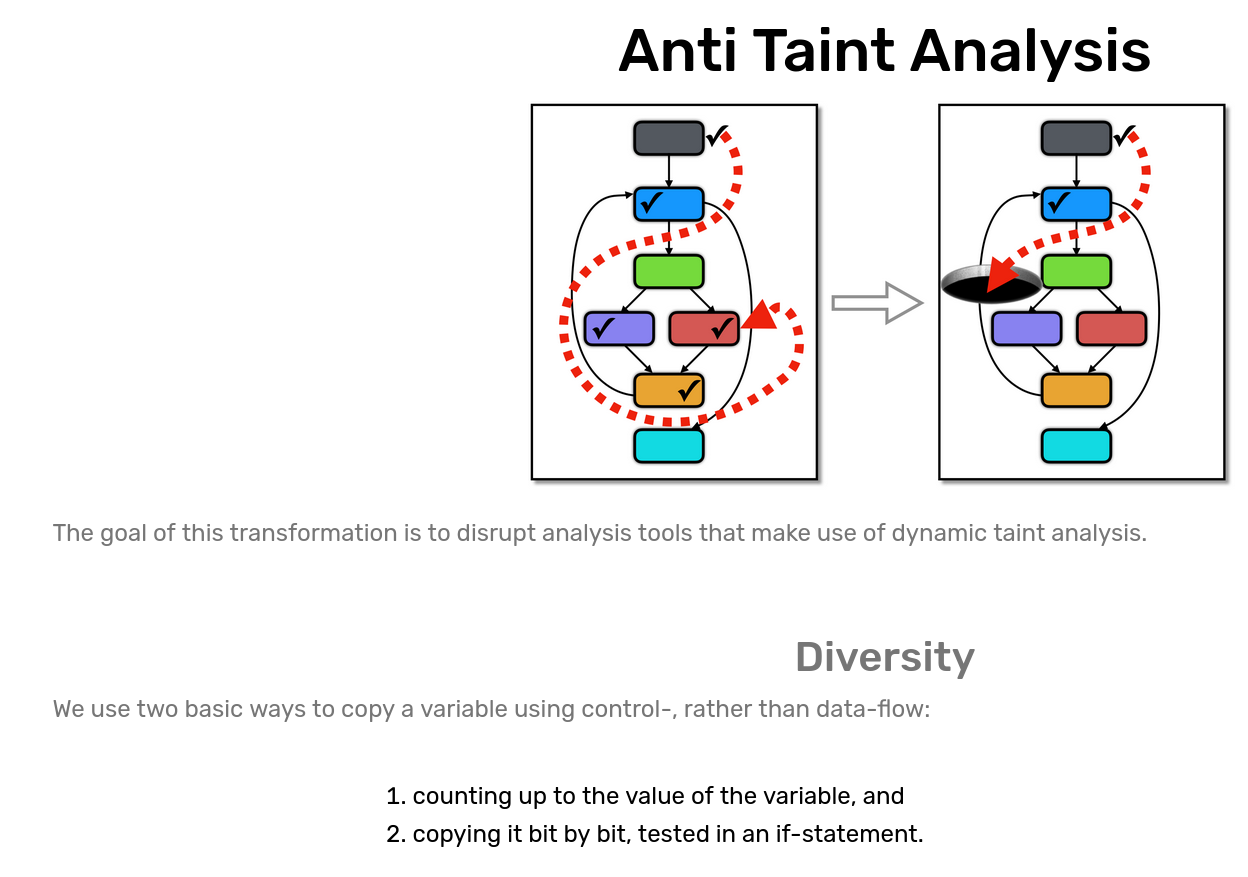
\includegraphics[height=0.9\textheight]{../taint/tigress-antitaint}
\end{frame}


\subsection{taint for finding mobile leaks}
\begin{frame}{example: TaintDroid}

\includegraphics[width=\textwidth]{../taint/taintdroid}
\end{frame}

\begin{frame}{TaintDroid instrumentation}
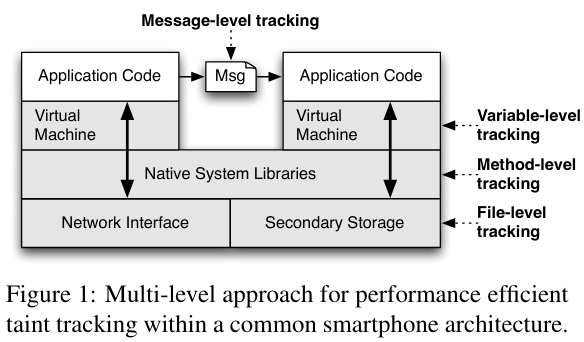
\includegraphics[height=0.9\textheight]{../taint/taintdroid-fig1}
\end{frame}

\begin{frame}{TaintDroid resutls}
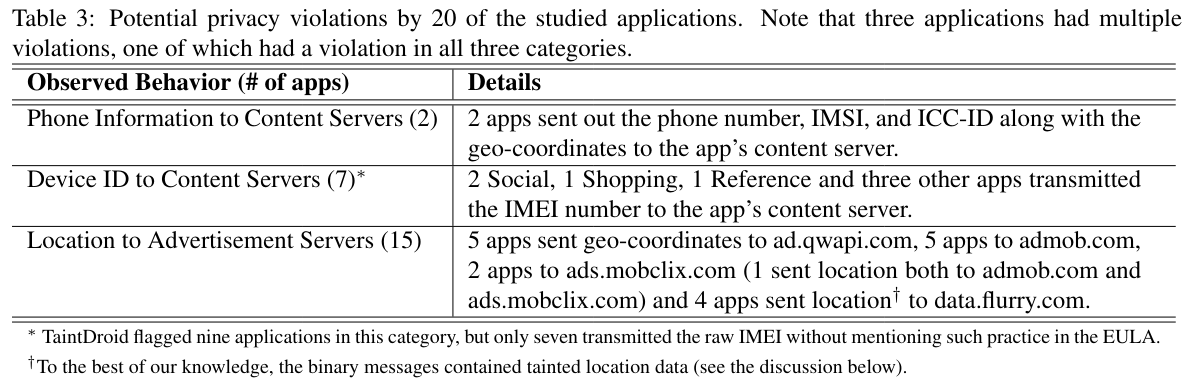
\includegraphics[width=\textwidth]{../taint/taintdroid-tbl3}
\end{frame}

\begin{frame}{TaintDroid and performance}
    \begin{itemize}
    \item modifying Dalvik ($\sim$ Java) VM allows good performance
    \item could do this sort of tracking on a ``live'' system
    \end{itemize}
\end{frame}



\section{next few topics}
\begin{frame}{logistics note}
    \begin{itemize}
    \item next few planned topics:
    \vspace{.5cm}
    \item (next) systems programming languages with memory safety (Rust as example)
    \item (after) sandboxing / privilege separation
        \begin{itemize}
        \item running code without trusting it as much
        \end{itemize}
    \item hardware support for memory safety + CFI (memory safety mitigation)
    \item concurrency bugs / time of check to time of use
    \vspace{.5cm}
    \item could make adjustments if there are topics people especially want
    \end{itemize}
\end{frame}

\section{Rust}

\subsection{aside: why do people like C/C++?}
\begin{frame}{why are people still using C/C++?}
    \begin{itemize}
    \item Python, Java, \ldots are great languages
    \item why are people using C, C++, etc.?
        \begin{itemize}
        \item which seem horrible for security?
        \end{itemize}
    \vspace{.5cm}
    \item history + good support
        \begin{itemize}
        \item lots of libraries in C, C++, \ldots
        \end{itemize}
    \item \myemph<2>{``zero overhead''}
        \begin{itemize}
        \item safe languages don't make it easy to get ``close to the machine''
        \item e.g. garbage collection overhead
        \item e.g. array checking overhead
        \end{itemize}
    \item no language VM --- easier to distribute
    \end{itemize}
\end{frame}

% FIXME

\subsection{safety + escape hatch}
\begin{frame}{safety rules + escape hatch}
    \begin{itemize}
    \item idea: can avoid out-of-bounds, etc. with safety rules
    \item \ldots but safety rules don't allow us to do some things fast
    \vspace{.5cm}
    \item so: have ``escape hatch'' to avoid safety checks in those cases
    \item hope: code that uses escape hatch can be tightly checked
        \begin{itemize}
        \item good target for expensive program analysis
        \end{itemize}
    \end{itemize}
\end{frame}



\begin{frame}[fragile,label=javaEscapeHatch]{Java: unofficial escape hatch}
    \begin{itemize}
    \item Oracle JDK and OpenJDK come with a class called \texttt{com.sun.Unsafe}
    \item Example methods:
    \end{itemize}
\begin{lstlisting}
public long allocateMemory(long size);
                        // returns pointer value
public void freeMemory(long address);
public long getLong(long address);
public void putLong(long address, long x);
\end{lstlisting}
    \begin{itemize}
    \item can be used to, e.g.,  write ``fast'' IntArray class
    \end{itemize}
\end{frame}


\begin{frame}{so, if Java has escape hatch\ldots}
    \begin{itemize}
    \item why do people not want to write \\ their performance-sensitive programs in Java?
    \vspace{.5cm}
    \item hard to integrate code that uses escape hatch with normal Java code
    \item hard to efficiently avoid dangling pointers when using escape hatch
        \begin{itemize}
        \item Is it safe to freeMemory from my FastIntArray class?
        \end{itemize}
    \item slow to pass garbage collected references to/from C/assembly code
    \item hard to avoid using garbage collector
        \begin{itemize}
        \item garbage collector performance can be variable
        \end{itemize}
    \end{itemize}
\end{frame}


\subsection{general philosophy}

\begin{frame}{Rust philosophy}
    \begin{itemize}
    \item default rules that only allow `safe' things
        \begin{itemize}
        \item no dangling pointers
        \item no out-of-bounds accesses
        \end{itemize}
    \item escape hatch to use ``raw'' pointers or unchecked libraries
    \item escape hatch can be used to write useful libraries
        \begin{itemize}
            \item e.g. Vector/ArrayList equivalent
            \item \myemph{expose interface that is safe}
        \end{itemize}
    \end{itemize}
\end{frame}



\section{backup slides}
\begin{frame}{backup slides}
\end{frame}

\subsection{static analysis limits?}
\begin{frame}{static analysis}
    \begin{itemize}
    \item need to avoid exploring way too many paths
        \begin{itemize}
        \item clang-analyzer: only a procedure at a time
        \item other analyzers: some way of pruning paths
        \end{itemize}
    \item need to avoid false positives
        \begin{itemize}
        \item probably can't always assume every if can be true/false
        \item one idea: apply symbolic-execution like techniques to prune
        \item clang-analyzer: limited by being procedure-at-a-time
        \end{itemize}
    \end{itemize}
\end{frame}



\end{document}
